\clearpage
\chapter{EXTRACTION OF BRUSH STROKES}
To generated bas-relief model from brush strokes,we need to first extract brush strokes.In this chapter, we demonstrate how to extract brush strokes from generated layers by modified Maximally Stable Extremal Regions (MSERs) algorithm, and we show that our optimization is more suitable for brush stroke extraction. In this chapter, the default MSERs algorithm and our modified algorithm are explained and their main characteristics compared. By successfully extract brush strokes, our algorithm can also be used in image editing,see section \ref{editing}.\\
The Maximally Stable Extremal Regions (MSERs) proposed in \cite{donoser2006efficient} and \cite{nister2008linear}for feature detection and image segmentation. A MSER is a 2D region detected by MSERs algorithm.  Generally,a brush stroke is considered as a closed stable region on paintings and it might be painted on different scales. MSERs have properties that form their superior performance as stable segmentation. The segmented MSER is closed under continuous geometric transformations and is invariant to affine intensity changes. Furthermore MSER are detected at different scales. So, we employ the Maximally Stable Extremal Regions (MSERs) proposed in \cite{donoser2006efficient} and \cite{nister2008linear} to extract brush strokes. MSERs algorithm requires a distinct difference between background and foreground while allowing a small variation of intensity within the selected stroke region. Usually, the brush strokes on the decomposed layers satisfy this requirement.
However, MSERs may fail in segmentation with the following scenarios,\\ 
(1) The brush stroke with the intensity very close to the background; \\
(2) Two adjacent brush stroke painted by different colors with the similar intensity;\\
(3) Overlapped brush strokes.\\
(4) Moreover, like the other existing segmentation approaches, the MSERs algorithm encounters over-segmentation issue as well. \\
To tackle these challenges, the coherent lines \cite{kang2007coherent} is introduced into MSERs, which both enhances the edges of strokes and preserves the completeness of strokes. For completeness sake, we briefly address MSERs algorithm and then address our modification.
\section{MSERs Algorithm}
MSERs can denote a set of distinguished regions that are detected in an intensity image. All of these regions are defined by an extremal property of the intensity function in the region and on its outer boundary, i.e. for a given extremal region S, the internal intensity is more than the intensity of boundary of S,

\[ \forall p \in S,\forall q \in \partial S , \longrightarrow I(p) \geq I(q)\]

where $\partial S $ denotes the boundary of $S$.$p$ and $q$ represent different pixels on the image, and $I(x)$ represent the intensity value of pixel $x$. 
Changing threshold, the extremal regions may further split or merge. The resulting extremal regions may be represented by the component tree. Accordingly, we may compute the change rate of the area of extremal region by

\[ \gamma(S_i^g) = \frac{\left ( \left |  S_j^{g-\Delta} \right |-\left |  S_k^{g+\Delta} \right | \right )}{\arrowvert S_i^g\arrowvert} \]

where $ \left | .  \right |$  denotes the cardinality, $ S_{i}^{g} $  is the i-th region which is obtained by thresholding at an intensity value g and $\Delta $ is a stability range parameter. $  g-\Delta $ and $ g+\Delta $ are obtained by moving upward and downward respectively in the component tree from the region $ S_{i} $ until a region with intensity value   or  is found. $ \left \{ i,j,k \right \}$ are the indices of nodes of the component tree. MSERs correspond to those nodes of the component tree that have a stability value $\gamma$, which is a local minimum along the path to the root of the tree.

\begin{figure}[H]
 	\centering
 	\begin{subfigure}[b]{0.4\textwidth}
		\centering
 		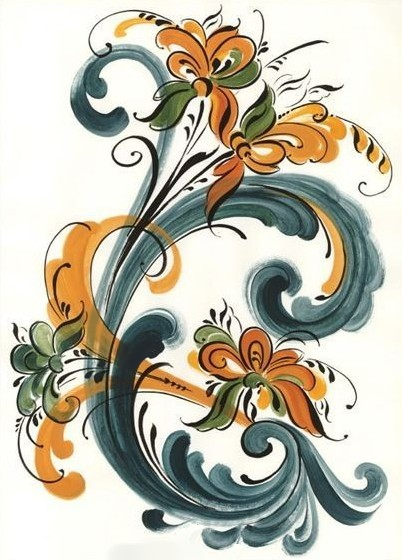
\includegraphics[width=\textwidth]{5.png}
 		\caption{input image}
 	\end{subfigure}
 		~  
 	\begin{subfigure}[b]{0.4\textwidth}
		\centering
	  	
\includegraphics[width=\textwidth]{inten_mser.png}
 		\caption{MSERs of the input image}	
 	\end{subfigure}
 	\label{modifi_mser}
	Perform the original MSERs on the intensity of image,different color indicates different regions.
\end{figure}



\section{Modified MSERs Algorithm}
\begin{figure}[H]
	\centering 
	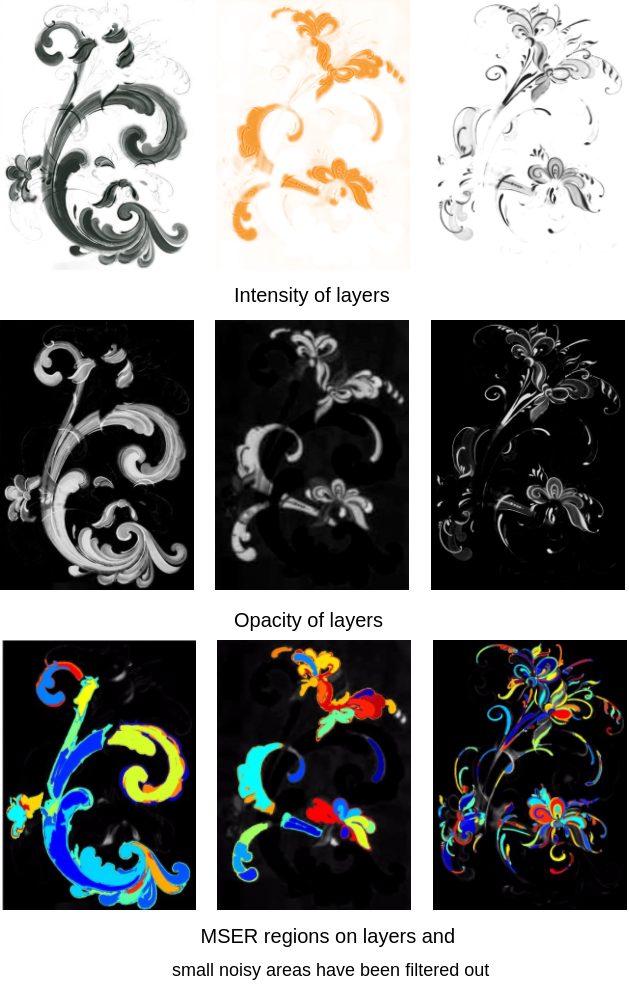
\includegraphics[width=10cm]{layer_sum.png}
	\caption{The opacity maps, and MSER regions of three layers by the modified MSERs.}
	\label{mser:alpha}
\end{figure}
In terms of the definition of the area change rate $\gamma$, MSERs may fail in segmentation with the following scenarios,\\
(1) The brush stroke with the intensity very close to the background; \\
(2) Adjacent brush strokes painted by different colors with the similar intensity;\\
(3) Overlapped brush strokes with different color.\\ 
(4) Moreover, like the other existing segmentation approaches, the MSERs algorithm encounters over-segmentation issue as well. 
\\
Comparing with default MSERs algorithm use intensity of input, our extraction is performed on opacity of generated layers.By doing so,in each layer, the opacity of the background is close to zero, which can be easily filter out, see Figure \ref{mser:alpha} , so, the first scenario can be handled. \\
The opacity of the brush strokes is always independent of the color,so two adjacent brush stroke painted by different colors would be separated into different layers, so,naturally,our extraction is suitable for the second scenario and third scenario, see Figure \ref{mser:alpha}. \\
Moreover, we perform the layer decomposition of Eq \ref{eq:layer_sum} on a brush painting and show the intensity and opacity of one layer associated with the individual histograms in Figure \ref{histo}. It can be noted that the opacity of the layer contains richer layered details than the intensity. So,our first modification is to perform MSERs on the opacity of every layer.\\
Secondly,we aim at the third scenarios of over-segmentation. When the extremal region is growing up through changing threshold, it is feasible to restrict the region by introducing the coherent lines. According to the definition of the extremal region, the boundary of region $S$ should satisfy,

\begin{equation*}
 \forall p \in S,\forall z \in   \bar{S} , \forall q \in \partial S \longrightarrow I(p) \geq I(q)  ~\mathrm{and}~  I(q) \leq I(z)
\end{equation*}
 
where $ \bar{S} $ denotes the complement of $S$. The second modification is to simply modify the opacity of layers, that is, overlapping the coherent lines with the layer and then changing the opacity of coherent lines to the smallest value in the layer.

To deal with the over-segmentation issue, the coherent lines play an important role. Given a region $S$, we modify the area change rate $\gamma$ as,
\begin{equation}
\gamma(S_i^g)=\frac{  \lvert \lvert S_j^{g-\Delta}\rvert -\lvert S_k^{g+\Delta} \rvert
	 \rvert     }{\arrowvert S_i^g\arrowvert} + \frac{  \lvert \lvert Q_j^{g-\Delta}\rvert -\lvert Q_k^{g+\Delta} \rvert
	 \rvert     }{\arrowvert Q_i^g\arrowvert} - (1-\frac{\lvert Q_i\rvert}{\lvert \partial S_i^g \rvert} )
\end{equation}


where $Q$ denotes the set of pixels which stay on the coherent lines and $Q \subset \partial S $. The third modification is to take into account the change of coherent lines to the boundary of $S$, i.e. the third term penalizes that a small portion of the boundary $\partial S$ is occupied by coherent lines.

Figure \ref{mser:alpha} shows the segmentation results by the modified MSERs, which correspond to brush strokes. It can be noted that performing MSERs on the intensity of image inevitable yields over-segmentations. Performing the modified MSERs on the opacity of layers, the strokes tend to complete and smooth within one layer. Moreover, some small regions with the distinct opacity values against neighboring areas have been filtered out, and no region is selected from background. 


\section{Image editing based on brush strokes}\label{editing}

Once the brushstrokes are extracted,we can simply recoloring strokes by assign a RGB value to the brushstroke while keep its opacity value.
Figure \ref{recoloring} a and \ref{recoloring} b shows recoloring strokes on three paintings respectively. As the strokes have been extracted, it is easy to separately recolor one or more strokes with different colors. However, for van Gogh oil painting, it seems tricky, since the painting is composed of lots of brushstrokes. Thus, we only recolor all the brushstrokes extract in one layer.
Moreover, Figure 10 further illustrates the brushstrokes of the van Gogh oil painting, which justifies the efficiency of our brushstroke extraction method.

Figure \ref{recoloring} c shows stroke manipulation through inserting objects . One of image editing tasks is to change a specified region with a new object in a seamless and effortless manner. Here we are interested in inserting new objects into a painting while keeping the transparency of the painting. Note that the inserted objects are opaque and are inserted between  brushstrokes here. The occluded regions of the objects are visible due to the transparency of the brushstrokes. Unlike the traditional image synthesis approaches, our implementation works on the strokes, which both guarantees seamless and keep the transparency of brushstrokes on the painting.


\begin{figure}[H]
	\centering
	\includegraphics[width=15cm]{recoloring.png}
	\caption{Image editing based on brush strokes}
	\label{recoloring}
	\medskip
Column a) shows 3 kinds of brush paintings, Chinese painting ,Rosemailing,and van Gogh oil painting . Column b) shows recoloring multiple strokes. Herein, for van Gogh oil painting, we show recoloring all the brushstrokes in one layer. Column c) shows inserting objects into these 3 paintings, in which the objects are opaque and are inserted in between brushstrokes.

\end{figure}

